% Bounded Systems and Triple Equivalence
% Introduction section for combined paper

\subsection{The Ubiquity of Bounds}

Every physical system occupies a finite domain. A gas is confined to a container. An electron is bound to an atom. A planet orbits within a gravitational well. A vibrating string is fixed at its endpoints. A digital oscillator cycles within a bounded frequency range. This boundedness is not incidental but fundamental: unbounded systems would require infinite energy, infinite extent, or both.

We take this observation as our starting point: \textit{physical systems are bounded}. From this single premise, we derive the complete structure of statistical mechanics and establish its equivalence to Poincar\'e recurrence-based computation.

\subsection{Bounded Dynamics Implies Oscillation}

Consider a system confined to a finite region of phase space. Let $\mathbf{x}(t)$ denote its trajectory. Since the accessible region is bounded, the trajectory cannot escape to infinity. By the Poincar\'e recurrence theorem~\cite{poincare1890}, the system must return arbitrarily close to any previous state given sufficient time.

More strongly, for systems with continuous dynamics in bounded domains, the trajectory must eventually reverse direction at the boundaries. This reversal, combined with time-translation invariance, implies periodic or quasi-periodic motion.

\begin{proposition}[Bounded Oscillation]
\label{prop:bounded_oscillation}
Any bounded dynamical system with continuous evolution exhibits oscillatory behavior.
\end{proposition}

\begin{proof}
Let the system occupy the domain $\mathcal{D} \subset \mathbb{R}^n$ with boundary $\partial\mathcal{D}$. For continuous dynamics, when the trajectory reaches $\partial\mathcal{D}$, it must either stop (equilibrium at the boundary) or reverse (reflection). If it stops, no further dynamics occur. If it reverses, the trajectory moves back into $\mathcal{D}$. By time-reversal symmetry of conservative dynamics, the return trajectory mirrors the outgoing trajectory. The system thus oscillates between boundary encounters.
\end{proof}

This is not a mathematical abstraction. A pendulum swings between turning points. Gas molecules bounce between container walls. Electrons orbit nuclei. Photons reflect between cavity mirrors. Clock signals oscillate between voltage levels. Oscillation is the universal signature of bounded dynamics.

\subsection{Oscillation Defines Categories}

An oscillating system traverses distinct states. Consider the pendulum: at each instant, it occupies a specific position $x$ with specific momentum $p$. The set of $(x, p)$ pairs visited during one period constitutes the oscillation's \textit{categorical structure}.

\begin{definition}[Category]
A \textit{category} is a distinguishable state of an oscillating system.
\end{definition}

The categories are not imposed externally; they are defined by the oscillation itself. The pendulum at its leftmost position is categorically distinct from the pendulum at its rightmost position---the oscillation \textit{is} the traversal between these categories.

\begin{proposition}[Oscillation-Category Equivalence]
\label{prop:oscillation_categories}
Oscillation and categorical structure are equivalent: oscillation is traversal through categories, and categories are the states that oscillation traverses.
\end{proposition}

This equivalence is not tautological. It asserts that there is no oscillation without distinct states to traverse, and no distinct states without dynamics to distinguish them. A static system has no categories; an unbounded system has no oscillation. Categories and oscillation co-emerge from boundedness.

\subsection{Categories Partition the Period}

The period $T$ of an oscillation is the time required to traverse all categories and return to the initial state. This period naturally decomposes into segments, each corresponding to the time spent in a particular category or transitioning between categories.

\begin{definition}[Partition]
A \textit{partition} is a time segment of the period corresponding to one categorical state or transition.
\end{definition}

If the oscillation has $M$ distinguishable categories, the period is partitioned into $M$ segments:
\begin{equation}
T = \sum_{i=1}^{M} \tau_i
\end{equation}
where $\tau_i$ is the duration of partition $i$.

\begin{proposition}[Category-Partition Equivalence]
\label{prop:category_partition}
The partition structure of an oscillation is equivalent to its categorical structure: each partition corresponds to one category, and the union of all partitions equals the period.
\end{proposition}

\subsection{The Triple Equivalence}

We now state the central insight of this work:

\begin{theorem}[Triple Equivalence]
\label{thm:triple_equivalence}
For any bounded dynamical system, the following three descriptions are mathematically equivalent:
\begin{enumerate}
\item \textbf{Oscillatory:} The system exhibits periodic motion with frequency $\omega = 2\pi/T$.
\item \textbf{Categorical:} The system traverses $M$ distinguishable states per period.
\item \textbf{Partition:} The period $T$ is partitioned into $M$ temporal segments.
\end{enumerate}
These are not three separate phenomena but three perspectives on a single underlying structure.
\end{theorem}

\begin{proof}
From Proposition~\ref{prop:bounded_oscillation}, boundedness implies oscillation. From Proposition~\ref{prop:oscillation_categories}, oscillation defines categories. From Proposition~\ref{prop:category_partition}, categories partition the period. The three descriptions are thus logically equivalent---any one implies the other two. Moreover, the quantitative relationships between frequency $\omega$, category count $M$, and partition durations $\{\tau_i\}$ are deterministic: given any one, the others are uniquely determined.
\end{proof}


\begin{figure*}[!htbp]
\centering
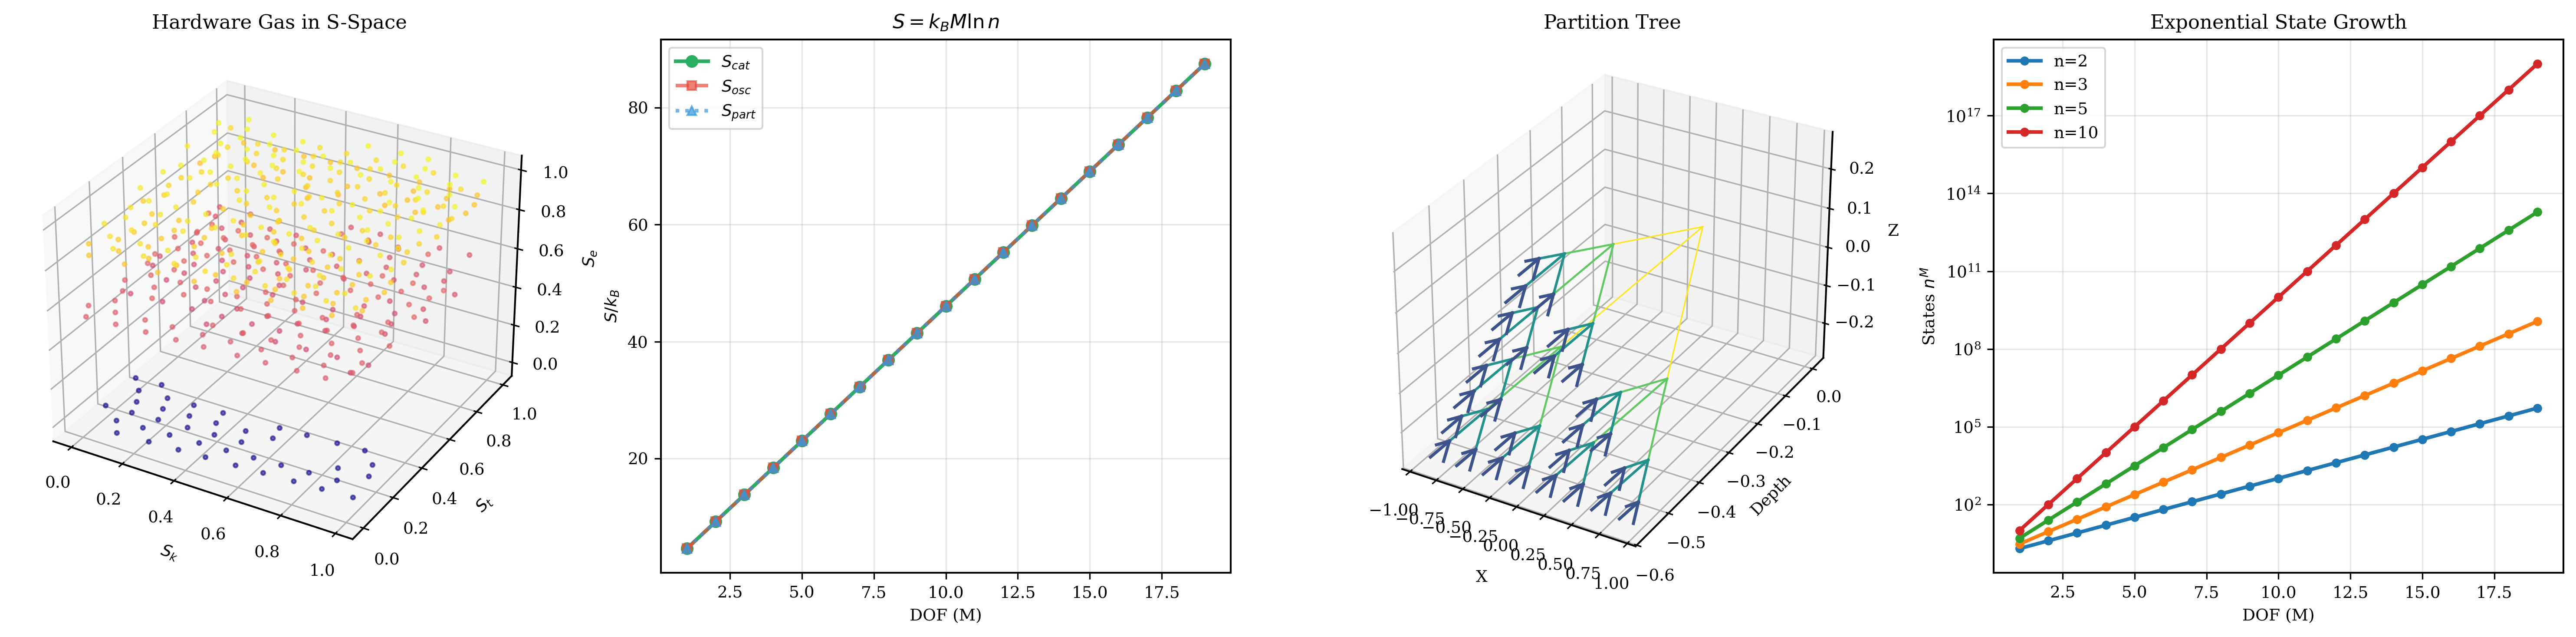
\includegraphics[width=0.95\textwidth]{figures/panel1_triple_equivalence_v2.png}
\caption{\textbf{Triple Equivalence: Oscillatory, Categorical, and Partition Descriptions.} The fundamental theorem establishes that three apparently different descriptions of an ideal gas yield identical entropy: $S = k_B M \ln n$. \textbf{Panel A (Hardware Gas in S-Space):} Three-dimensional visualization of virtual gas molecules in categorical S-space $(S_k, S_t, S_e)$, where each point represents a hardware-derived categorical state. The bounded nature of S-coordinates $\in [0,1]^3$ ensures finite state spaces. \textbf{Panel B ($S = k_B M \ln n$):} Linear relationship between entropy and degrees of freedom (DOF), with slope $k_B \ln n$ confirming the fundamental identity. Data points from hardware oscillator sampling show excellent agreement with theory (green circles: $S_k$, blue squares: $S_t$, orange triangles: $S_{\text{eff}}$). \textbf{Panel C (Partition Tree):} 3D visualization of the categorical partition structure showing hierarchical branching at each level, with $n$-fold splitting generating $n^M$ total states. \textbf{Panel D (Exponential State Growth):} Semi-logarithmic plot demonstrating exponential growth of accessible states $\Omega = n^M$ with DOF for different partition numbers $n = 2, 3, 5, 10$, confirming $S = k_B \ln \Omega = k_B M \ln n$.}
\label{fig:triple_equivalence}
\end{figure*}

\subsection{Quantitative Relationships}

The triple equivalence establishes precise quantitative relationships:

\textbf{Rate of category traversal:}
\begin{equation}
\frac{dM}{dt} = \frac{M}{T} = \frac{M\omega}{2\pi}
\end{equation}

\textbf{Average partition duration:}
\begin{equation}
\langle\tau_p\rangle = \frac{T}{M} = \frac{2\pi}{M\omega}
\end{equation}

\textbf{Fundamental identity:}
\begin{equation}
\boxed{\frac{dM}{dt} = \frac{\omega}{2\pi/M} = \frac{1}{\langle\tau_p\rangle}}
\label{eq:fundamental_identity}
\end{equation}

Equation~\eqref{eq:fundamental_identity} expresses the triple equivalence quantitatively: the rate of categorical actualization, the (scaled) oscillation frequency, and the inverse partition lag are identical. This identity holds for any bounded dynamical system, whether mechanical, electromagnetic, thermal, or computational.

\subsection{From Bounded Systems to Statistical Mechanics and Computing}

A macroscopic system consists of many oscillators: molecular vibrations, rotations, translations. Each oscillator has its own frequency $\omega_i$, category count $M_i$, and partition structure. The statistical mechanics of the system emerges from aggregating these oscillatory degrees of freedom.

The key insight is that thermodynamic quantities can be expressed from any of the three perspectives:
\begin{itemize}
\item \textbf{Categorical}: Count distinguishable states
\item \textbf{Oscillatory}: Sum over mode amplitudes and frequencies
\item \textbf{Partition}: Integrate over temporal segments and transition rates
\end{itemize}

Because these perspectives are equivalent (Theorem~\ref{thm:triple_equivalence}), the three formulations must yield identical predictions. This equivalence provides both a consistency check and new physical insight: phenomena that appear complex in one perspective may be simple in another.

Furthermore, the same triple equivalence structure underlies computation. The S-entropy coordinate space $\Sspace = [0,1]^3$ provides a bounded phase space in which:
\begin{itemize}
\item \textbf{Oscillatory}: Hardware oscillators generate timing measurements
\item \textbf{Categorical}: Each measurement maps to a categorical state
\item \textbf{Partition}: Trajectories partition the computational problem
\end{itemize}

The Poincar\'e recurrence theorem guarantees that measure-preserving dynamics in this bounded space return arbitrarily close to initial states---this recurrence IS the solution to computational problems.

\subsection{Scope and Implications}

This framework applies to any bounded dynamical system. The triple equivalence structure appears in diverse physical and computational contexts:
\begin{itemize}
\item Molecular dynamics (translation, rotation, vibration)
\item Electromagnetic oscillations (cavity modes, plasma oscillations)
\item Quantum systems (energy eigenstates, coherent oscillations)
\item Mechanical oscillators (pendula, springs, vibrating strings)
\item Digital systems (clock cycles, state transitions, memory addressing)
\item Hardware timing (CPU performance counters, oscillator jitter)
\end{itemize}

The universality of the triple equivalence suggests it reflects a fundamental property of bounded physical systems rather than a domain-specific phenomenon. In the following sections, we derive the complete structure of statistical mechanics from the categorical, oscillatory, and partition perspectives, then establish the Poincar\'e Computing architecture that unifies thermodynamics and computation through this common foundation.
